\documentclass[11pt]{article} % 
\usepackage[pdftex]{graphicx}
\usepackage{fullpage}
\usepackage{graphicx}
\usepackage{graphics}
\usepackage{psfrag}
\usepackage{pgf}
\usepackage{color}
\usepackage{tikz}
\usetikzlibrary{arrows,automata}
\usepackage[latin1]{inputenc}
\usepackage{amsthm}
\usepackage{amsmath,amssymb}
\usepackage{enumerate}
\setlength{\textwidth}{6.5in}
\setlength{\textheight}{9in}
\newcommand{\N}{\mathbb{N}}
\newcommand{\Z}{\mathbb{Z}}
\newcommand{\R}{\mathbb{R}}
\newcommand{\Q}{\mathbb{Q}}
\newcommand{\C}{\mathbb{C}}
\newcommand{\PP}{\mathbb{P}}
\newcommand{\tab}{\;\;\;\;\;}
\newcommand{\inv}{^{-1}}
\newcommand{\tr}{\textrm}
\newcommand{\lc}{\sqcup}
\newcommand{\var}{\tr{Var}}
\newcommand{\cov}{\tr{Cov}}
\newcommand{\like}{\mathcal{L}}

\begin{document}

\hfill Robert Johns

\hfill March 27, 2014

\begin{center} {\Large CSCI 678: Statistical Analysis of Simulation Models}\\{\large Homework 9}\end{center}

\begin{enumerate}

%%%%%
%1
\item Let us expand the computational formula $y_t = \alpha x_t + (1 - \alpha)y_{t-1}$ recursively to see if we arrive at the filter.

\begin{align*}y_t &= \alpha x_t + (1 - \alpha)y_{t-1} \\
&= \alpha x_t + (1 - \alpha)(\alpha x_{t-1} + (1 - \alpha)y_{t - 2})\\
&= \alpha x_t + \alpha(1 - \alpha)x_{t-1} + (1 - \alpha)^2y_{t-2}\\
&= \alpha x_t + \alpha(1 - \alpha)x_{t-1} + (1 - \alpha)^2(\alpha x_{t-2} + (1-\alpha)y_{t-3})\\
&= \alpha x_t + \alpha(1 - \alpha)x_{t-1} + \alpha(1 - \alpha)^2x_{t-2} + (1-\alpha)^3y_{t-3}
\end{align*}

A pattern emerges; we see that we can express the recursion above with the infinite sum:
$$y_t = \sum_{r = 0}^\infty \alpha(1 - \alpha)^rx_{t - r}$$
or, equivalently:
$$y_t = \sum_{r = -\infty}^0\alpha(1-\alpha)^{-r}x_{t+r}$$

%%%%%
%2
\item First, we convolute $\left(\frac{1}{4}, \frac{1}{4}, \frac{1}{4}, \frac{1}{4}\right)$ and $\left(\frac{1}{4}, \frac{1}{4}, \frac{1}{4}, \frac{1}{4}\right)$.

We get $\left(\frac{1}{4} * \frac{1}{4}, \frac{1}{4} * \frac{1}{4} + \frac{1}{4} * \frac{1}{4}, \frac{1}{4} * \frac{1}{4}\right) = \left(\frac{1}{16}, \frac{1}{4}, \frac{1}{16}\right)$.  

We then convolute that with $\left(\frac{1}{5}, \frac{1}{5}, \frac{1}{5}, \frac{1}{5}, \frac{1}{5}\right)$.

We get $\left(\frac{1}{16} * \frac{1}{5}, \frac{1}{16} * \frac{1}{5} + \frac{1}{4} * \frac{1}{5}, \frac{1}{16} * \frac{1}{5} + \frac{1}{4} * \frac{1}{5} + \frac{1}{16} * \frac{1}{5}\right) = \left(\frac{1}{80}, \frac{3}{80}, \frac{3}{40}\right)$.

We then convolute that with $\left(-\frac{3}{4}, \frac{3}{4}, 1, \frac{3}{4}, -\frac{3}{4}\right)$.

We get $\left(-\frac{3}{4} * \frac{1}{80}, \frac{3}{4} * \frac{1}{80} - \frac{3}{4} * \frac{3}{80}, 1* \frac{1}{80} + \frac{3}{4} * \frac{3}{80} - \frac{3}{4} * \frac{3}{40}\right) = \frac{1}{320}\left(-3, -6, -5\right)$

%%%%%
%3
\item \begin{enumerate}

%3a
\item$\\$ 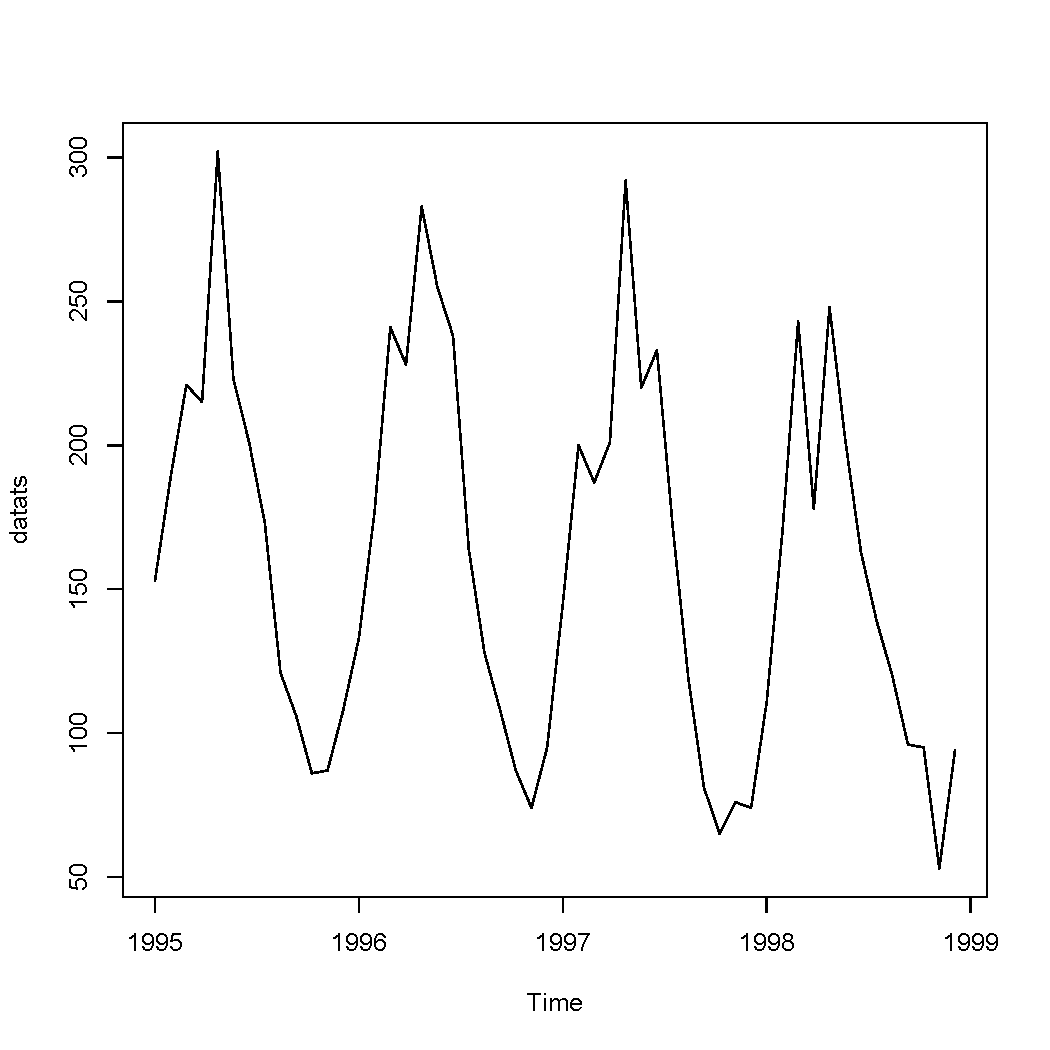
\includegraphics[scale = .4]{plot1.pdf}

%3b
\item The trend appears to be negative and linear.  Seasonally, each year begins part of the way up a steep climb, followed by a short fall and a quick recovery, peaking around a third of the way unto the year, falling again until shortly before the next year, at which time the data will climb again into a new year. 

\end{enumerate}

%%%%%
%4
\item \begin{enumerate}

%4a
\item $\\$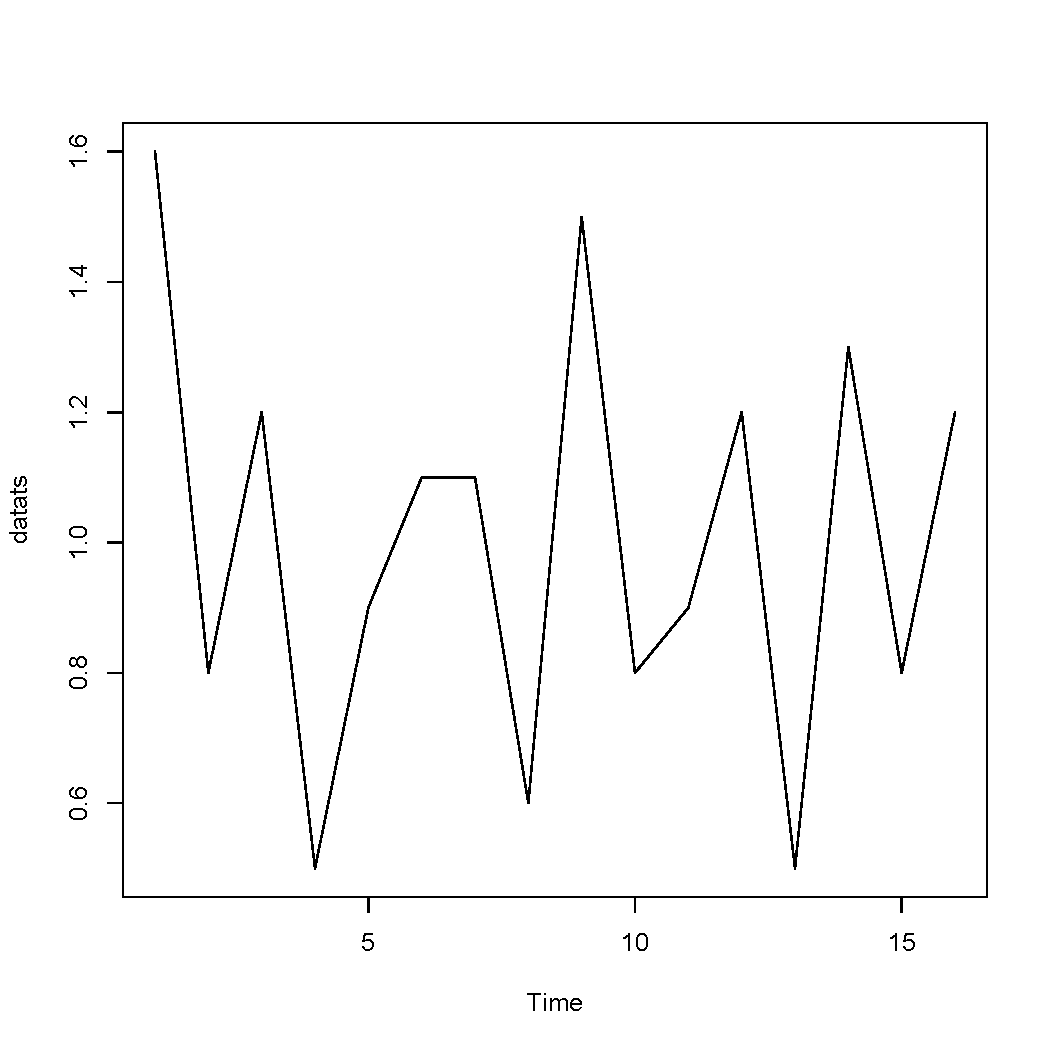
\includegraphics[scale = .4]{plot2.pdf}

%4b
\item The mean value of the time series is 1.  Each value seems to be on the opposite side of the mean from the successive value, so it will be negative.  To hazard a guess, I'd say around $-0.5$.

%4c
\item $\\$ 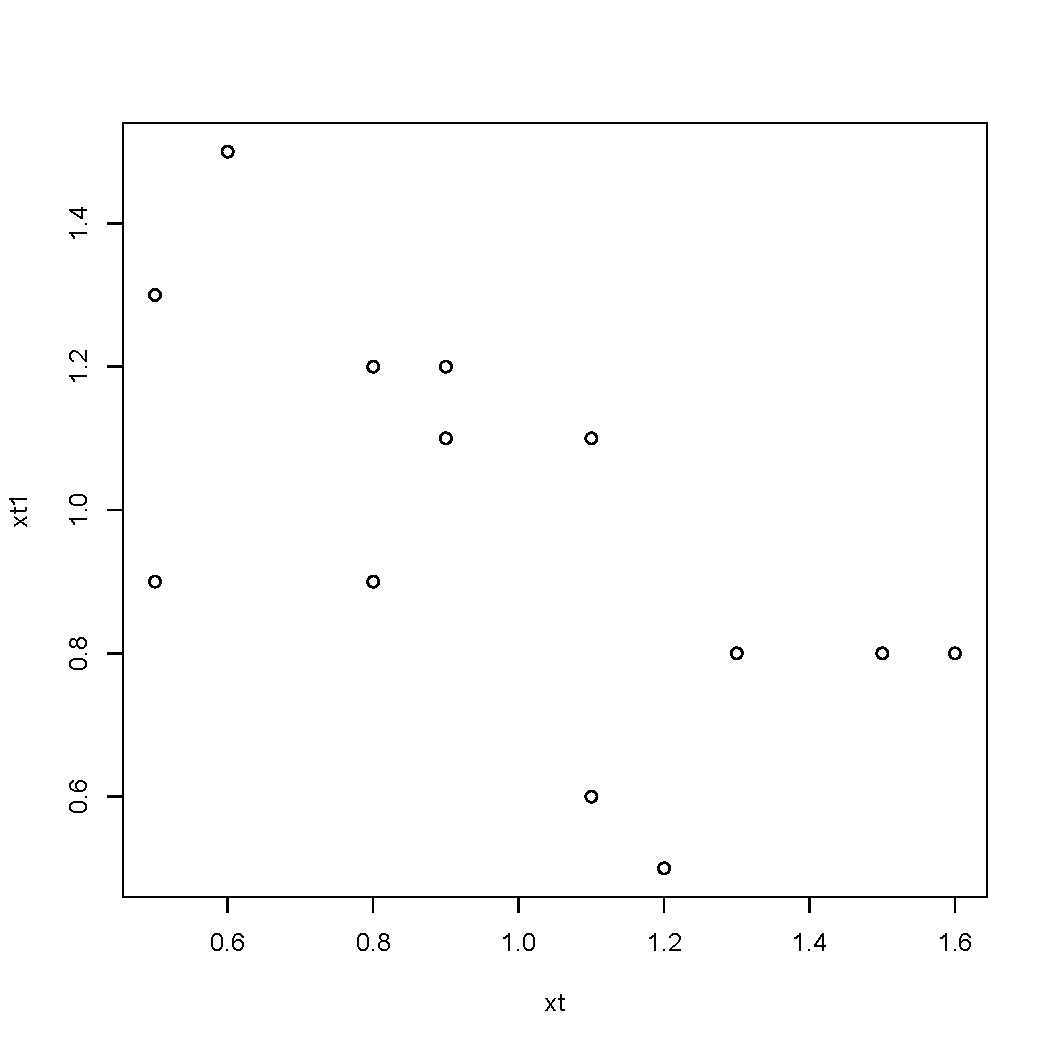
\includegraphics[scale = .4]{plot3.pdf}

A regression line with a slope of a little less than $-.5$ would fit the data reasonably well, so I'll update my guess to $-.6$

%4d
\item The R program \texttt{asm9b.r} was used to calculate the result.  It gives: $-.641052$

%4e
\item The R program \texttt{asm9b.r} was used to calculate the result.  It gives: $-0.5853659$
 
%4f
\item The R program \texttt{asm9b.r} was used to calculate the result.  It gives: $-0.5487805$

%4g
\item The R program \texttt{asm9b.r} was used to calculate the result.  It gives: $-0.5853659$

%4h
\item The R program \texttt{asm9b.r} was used to calculate the result.  It gives:

$\begin{array}{| l | r |}\hline
\tr{lag} & \tr{result}\\\hline
1 & -0.5487805\\
2 & 0.25\\
3 & -0.1036585\\
4 & -0.1646341\\
5 & 0.06707317\\
\hline\end{array}$

%4i
\item The R program \texttt{asm9b.r} was used to calculate the result.  It gives:

$\begin{array}{| l | r |}\hline
\tr{lag} & \tr{result}\\\hline
1 & -0.8645833\\
2 & -1.965278\\
3 & 0.1138117\\
4 & -1.527006\\
5 & -0.2843364\\
\hline\end{array}$

\end{enumerate}

%%%%%
%5
\item All computations were done using the R program \texttt{asm9c.r}.  The plot of the time series is:

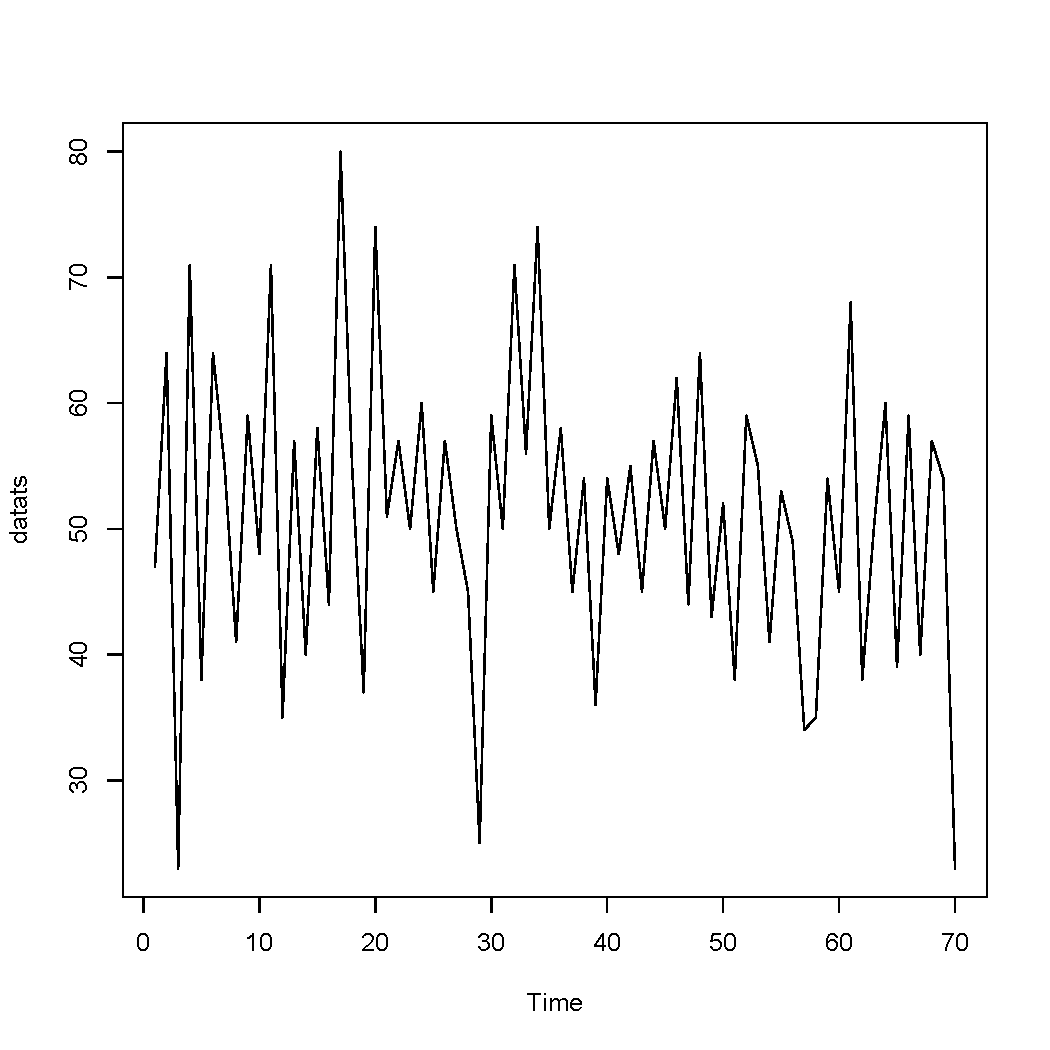
\includegraphics[scale = .4]{plot4.pdf}

The plot of the autocorrelation function is as follows (95\% confidence limits dashed lines): 

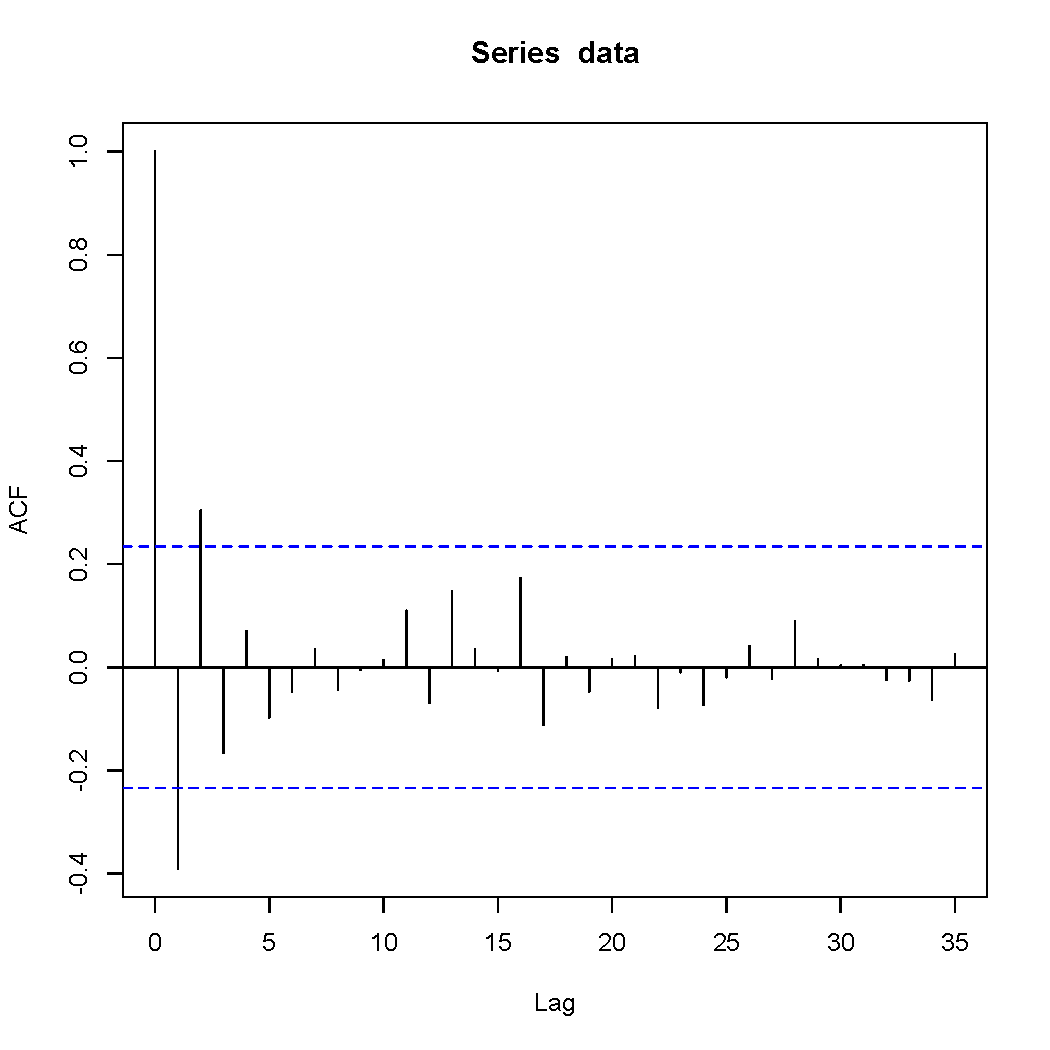
\includegraphics[scale = .4]{plot5.pdf}

The values for the autocorrelation function are:
\begin{verbatim}     0      1      2      3      4      5      6      7      8      9 
 1.000 -0.390  0.304 -0.166  0.071 -0.097 -0.047  0.035 -0.043 -0.005 
    10     11     12     13     14     15     16     17     18     19 
 0.014  0.110 -0.069  0.148  0.036 -0.007  0.173 -0.111  0.020 -0.047 
    20     21     22     23     24     25     26     27     28     29 
 0.016  0.022 -0.079 -0.010 -0.073 -0.020  0.041 -0.022  0.089  0.016 
    30     31     32     33     34     35 
 0.004  0.005 -0.025 -0.026 -0.063  0.026 \end{verbatim}

From this plot, we see that the data until lag 10 is correlated normally (damping to 0), but subsequent lags have stronger correlation, for example, the spike near lag 16 and again near 30.  This, to me, is very unusual, because you would expect the data to decrease in correlation as time increases, especially considering this time series appears very random, with no obvious trend.  Perhaps this indicates some seasonal behavior with a observational period near 15.

%%%%%
%6
\item I was born in 1992, so I chose to start the data in January of that year.  It won't affect the data in any way, I just though it'd be fun.  The quarterly results are:
\begin{verbatim}         Qtr1     Qtr2     Qtr3     Qtr4
1992 44.66667 57.66667 51.66667 51.33333
1993 51.66667 59.66667 54.00000 55.66667
1994 50.66667 43.00000 59.00000 60.66667\end{verbatim}

\end{enumerate}

\line(1,0){470}

Project Synopsis: I intend to focus my project on the midsquare method of random number generation.  I will go through the history of the method in-depth, focusing on the method's faults.  I will then present some researched improvements on the method that avoid those pitfalls.

\end{document}